\newpage
\section{Crystal Structure of Sodium Chloride (NaCl)}
\label{sec:NaCl}

\subsection*{Structural Analysis}

The following plot shows the obtained intensity distribution.

\begin{figure}[h]
    \centering
    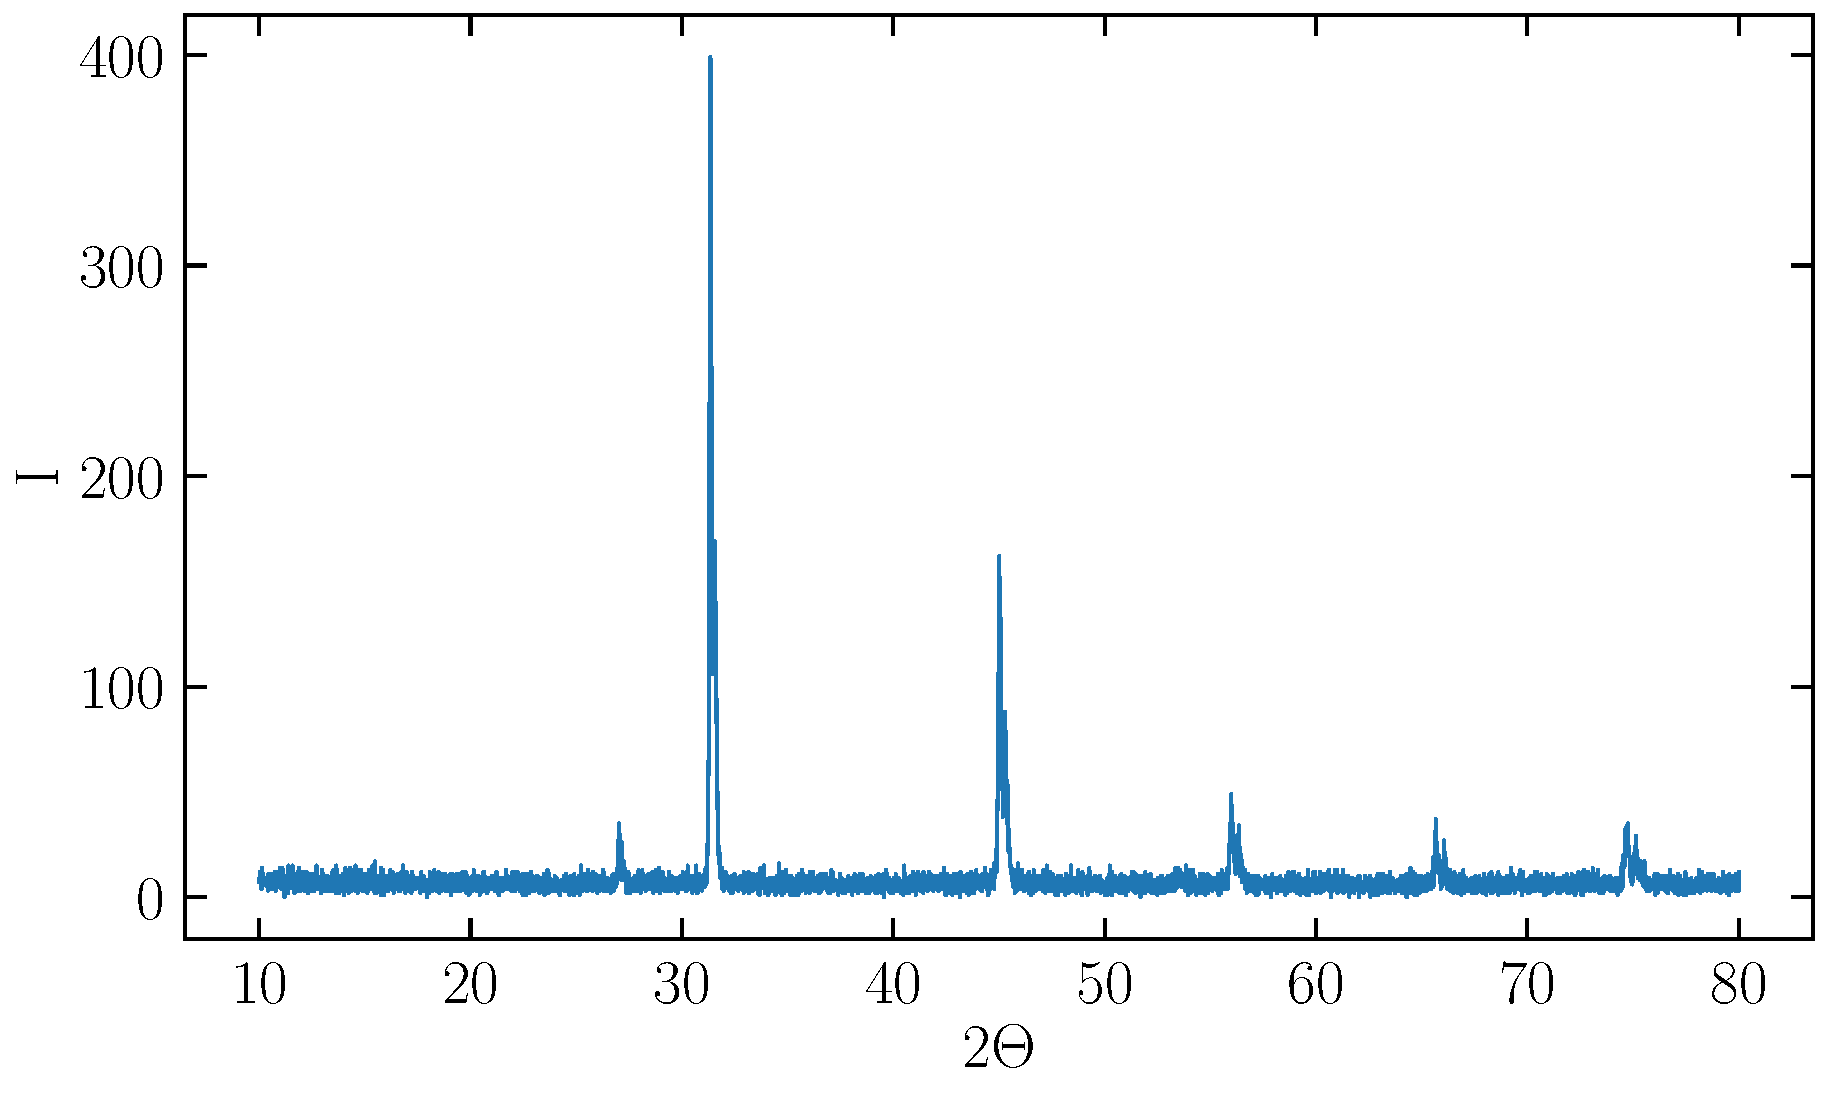
\includegraphics[width=\textwidth]{Pictures/Evaluation/42/IntDistNaCl.pdf}
    \caption{Intensity distribution of the NaCl experiment.}
\end{figure}

\begin{table}[ht]
    \centering
    \begin{tabular}{c|c c c}
        \hline
        Peak No. &  2$\theta_{fit}$ / \SIUnitSymbolDegree &  $I_{fit}$ / a.u. &   $FWHM$ / \SIUnitSymbolDegree \\
        \hline
            1 &    27.15 &   0.05 &  0.11 \\
            2 &    31.48 &   0.86 &  0.12 \\
            3 &    45.02 &   0.48 &  0.16 \\
            4 &    53.62 &   0.03 &  0.18 \\
            5 &    56.21 &   0.15 &  0.19 \\
            6 &    65.66 &   0.10 &  0.22 \\
            7 &    72.70 &   0.02 &  0.24 \\
            8 &    74.70 &   0.17 &  0.25 \\
        \hline
    \end{tabular}
    \caption{Fit values for each peak in the intensity distribution.}
    \label{tab:fitVals}
\end{table}


